\chapter{Methodik}
\label{chap:methodik}

In diesem Kapitel wird der methodische Aufbau dieser Thesis beschrieben und begründet.
Die Arbeit ist als industrielle Fallstudie in Zusammenarbeit mit \emph{levigo solutions} konzipiert und dient der Evaluation des \gls{mmf} an einer bestehenden Microservices-Architektur.
Diese Fallstudie besteht aus zwei Hauptbestandteilen.
Im ersten Teil wird ein Refactoring des Produktes \emph{jadice flow} nach Anleitung des Frameworks durchgeführt.
Im zweiten Teil wird das Ergebnis dieses Refactorings verwendet, um eine Evaluation des Frameworks und Werkzeugs abzuschließen.

\section{Refactoring mit \gls{mmf}}

Die Vorgehensweise beim Refactoring ist durch das Framework sehr genau vorgegeben.
Daher wird das Refactoring in dieser Thesis in die gleichen drei Phasen unterteilt wie in \cref{sec:mmf} beschrieben.
In der ersten Phase wird gemeinsam mit den Stakeholdern des Produkts ein Architekturreview nach \Citet{SVAHNBERG20071893} durchgeführt.
Diese Methode wird in \cref{sec:methodik-architekturreview} näher beschrieben.
Das wesentliche Ergebnis dieses Reviews sind die gewünschten \glspl{qa} des Systems.
Diese Attribute sind die Basis für Phase 2 und 3 und werden in den \gls{arh} eingegeben.
Dieser führt Berechnungen mit den \glspl{qa} durch und kann so eine Liste von Refactoring-Methoden vorschlagen, die nach ihrer Eignung für die \glspl{qa} sortiert sind.
Als weitere Eingabe dafür dienen bestimmte Filter, die in \cref{sec:durchführung-phase2} näher erläutert werden.
Aus der resultierenden Liste von Migrationsmethoden werden die besten Vorschläge betrachtet und bewertet, bevor einer davon ausgewählt und in den folgenden Phasen verwendet wird.
Analog dazu wird in Phase 3a auf Basis der \glspl{qa} und Filter aus Phase 2 eine sortierte Liste von Patterns und Best Practices vorgeschlagen.
Das Vorgehen bei der Auswahl der Filter sowie die spätere Inspektion der Vorschläge des \gls{arh} werden in Form von strukturierten Feldnotizen protokolliert.
Deren genauere Funktion und Form dieser wird in \cref{sec:structured-field-notes} näher erläutert.

\subsection{Architekturreview}
\label{sec:methodik-architekturreview}

Die Methodik eines Architekturreviews wird in dieser Thesis nach Vorschlag des \gls{mmf}/\gls{arh} dazu verwendet, Qualitätsanforderungen an das System, sogenannte \acrfullpl{qa}, zu sammeln.
Für Konformität mit dem Werkzeug \gls{arh}, das als Ergebnis des Architekturreviews Szenarien benötigt, die \acrfullpl{qa} beschreiben, beschränkt sich die Auswahl möglicher Verfahren für die erste Phase auf Szenarien-basierte Architekturreviews.
Das bedeutet, dass die gewünschten \glspl{qa} des Systems in Form von Szenarien erfasst und dokumentiert werden.
Ein Szenario beschreibt dabei eine Interaktion eines Stakeholders mit dem Produkt \cite{kazman_2000}.
Diese Konkretisierung von Qualitäten soll vor allem die Verständlichkeit fördern. 
Dabei werden mit jedem Szenario zugehörige \glspl{qa} assoziiert, wodurch am Ende eine Abbildung aller \glspl{qa} auf ihre Priorität möglich ist.
Diese Abbildung ist das eigentliche Ergebnis, das der \gls{arh} als Eingabe für die weiteren Phasen benötigt.
Die Szenarien sind dabei lediglich ein Zwischenprodukt und sollen dabei helfen, eine genauere Vorstellung davon zu bekommen, welche spezifischen Situationen mit den \glspl{qa} verbunden sind.
Sie ermöglichen auch eine Bewertung der Wichtigkeit und technischen Schwierigkeit anhand konkreter Situationen, was bei abstrakten \glspl{qa} schwieriger wäre.

Folgend werden verschiedene akademische Methoden beschrieben und verglichen und anschließend die verwendete Methode als Abwandlung dieser Methoden erläutert.

\subsubsection{Vergleich verschiedener Methoden}
\label{sec:atam-saam-svahnberg}

Geläufige Szenarien-basierte Verfahren sind die \gls{saam} nach \Citet{saam} und die \gls{atam} nach \Citet{kazman_2000}.
\gls{atam} ist der Nachfolger und eine Überarbeitung von \gls{saam}, weshalb folgend lediglich \gls{atam} näher betrachtet wird.
Die Autoren beschreiben mit \gls{atam} eine Methode, die aus insgesamt neun Schritten besteht.
Diese Schritte sollen mit den Stakeholdern des Produkts innerhalb von drei Arbeitstagen durchgeführt werden.
Da das Ausmaß dieser allerdings nicht angemessen für den Rahmen einer Thesis ist \cite{master-marvin-knodel}, würde für diese Arbeit höchstens eine stark abgewandelte Version dieser infrage kommen.
Stattdessen wurde sich in dieser Thesis für eine Modifikation des Architekturreviews nach \Citet{SVAHNBERG20071893} entschieden.
Es handelt sich dabei ebenfalls um eine Szenarien-basierte Methode, die auf \gls{saam} und \gls{atam} basiert, jedoch spezieller für kleinere Anwendungsfälle entwickelt wurde.
Die Autoren erläutern die Verwendung dieser zur Evaluation von Studentenprojekten, die ein reales Softwareentwicklungsprojekt mit Industriekunden simulieren und einen Rahmen von 10-15 Teilnehmern und 20 Wochen Arbeitszeit vorsehen.

\subsubsection{Architekturreview nach \Citet{SVAHNBERG20071893}}

Das Architekturreview nach  \Citet{SVAHNBERG20071893} umfasst sechs Schritte (Übersicht in \cref{tab:svahnberg-plan}).
\begin{table}[!h]
  \centering
  \begin{tabular}{l l}
    \toprule
    \textbf{Aktivität} & \textbf{Zeit (in Minuten)} \\ \midrule
    1. Einleitung in das Projekt & 15 \\
    2. Identifikation von Qualitätsanforderungen & 20 \\
    3. Szenarienerhebung & 45 \\
    ~~~~Pause & 20 \\
    4. Architekturpräsentation & 20 \\
    5. Szenario- und Architekturanalyse & 90 \\
    6. Fazit & 15 \\
    \bottomrule
  \end{tabular}
  \caption[Zeitplan für ein Architekturreview nach \Citet{SVAHNBERG20071893}]{
    Zeitplan für ein Architekturreview nach \Citet{SVAHNBERG20071893}.
  }
  \label{tab:svahnberg-plan}
\end{table}

Diese sollen in einer etwa vierstündigen, mo\-de\-rierten Gruppendiskussion mit den wichtigsten Stakeholdern des Produkts durchgeführt werden.
Im ersten Schritt gibt der \gls{po} eine Einführung in das Projekt, in der Ziele für das Produkt sowie die Organisation geschildert werden.
Im zweiten Schritt wird in einer Brainstorming-Runde zusammen mit dem \gls{po}, End-Nutzern und Architekten die Identifikation von \glspl{qa} durchgeführt.
Hierfür dient die Liste der Qualitätskriterien gemäß ISO 9126~\cite{ISO-9126} als Vorlage für mögliche \glspl{qa}.
Im dritten Schritt ordnen \gls{po} und End-Nutzer die Liste der \glspl{qa} nach ihrer Wichtigkeit und fügen den drei wichtigsten jeweils zwei Szenarien hinzu.
Nach einer Pause präsentiert im vierten Schritt ein Softwarearchitekt die vorgeschlagene Architektur.
Anschließend werden im fünften Schritt die Szenarien sequenziell analysiert und bewertet, inwiefern sie durch die Architektur erfüllt werden und wo etwaige Probleme bestehen.
Im sechsten Schritt werden alle identifizierten Probleme und Aspekte, die mehr Aufmerksamkeit benötigen, final diskutiert und der gesamte Prozess zusammengefasst.

\subsubsection{Anpassung des Architekturreviews auf den \gls{arh}}

Ein volles Architekturreview, auf Deutsch auch mit Architekturbewertung zu übersetzen, ist generell bei der Verwendung des \gls{arh} und somit in dieser Thesis nicht das primäre Ziel.
Vielmehr entfällt das Hauptziel eines herkömmlichen Architekturreviews: die Bewertung.
Stattdessen wurde die in \cref{tab:architekturreview-plan} dargestellte Methodik zur Extraktion von Szenarien und \glspl{qa} entworfen.
\begin{table}[!h]
  \centering
  \begin{tabular}{m{4cm} m{8cm} p{1.3cm}}
    \toprule
    \textbf{Schritt nach \Citet{SVAHNBERG20071893}} & \textbf{Sub-Schritt} & \textbf{Zeit} \\ \midrule
    1. Einleitung in die Me\-tho\-dik & & 10 min\\ \hline
    \multirow{2}{=}[0cm]{2. Identifikation von Qualitätsanforderungen} & Umfrage über wichtigste drei Sub-\glspl{qa} &  \multirow{3}{=}[0.2cm]{20 min}\\
    & Diskussion über Priorisierung der Sub-\glspl{qa} & \\ \hline
    \multirow{3}{=}[-0.3cm]{3. Szenarienerhebung} & Erstellen Szenarien zu wichtigsten Sub-\glspl{qa}& \multirow{3}{=}[-0.3cm]{60 min}\\
    & Hinzufügen Wichtigkeit \& Technische Schwierigkeit zu Szenarien  & \\
    & Szenarien mit weiteren \glspl{qa} assoziieren  & \\ \hline
    5. Szenario- und Archi\-tek\-turanalyse & Architekturbewertung anhand der Szenarien & 10 min \\
    \bottomrule
  \end{tabular}
  \caption[Zeitplan für das Architekturreview]{
    Zeitplan für das Architekturreview in Phase 1 dieser Thesis.
  }
  \label{tab:architekturreview-plan}
\end{table}


Wie in der Tabelle angemerkt, dienen als Vorlage für die Methodik die ersten Schritte des Architekturreviews nach \Citet{SVAHNBERG20071893}.
Außerdem werden auch einzelne Aspekte von \gls{atam} \cite{kazman_2000} verwendet.
Die einzelnen Schritte werden folgend näher beschrieben.

Im ersten Schritt ist die Einleitung in die Methodik geplant.
Dabei handelt es sich um eine Modifikation des nach \Citet{SVAHNBERG20071893} geplanten ersten Schritts, bei dem stattdessen eine Einleitung in das Projekt erfolgt.
Dieser stammt vermutlich aus dem Kontext der Studentenprojekte, bei denen mehrere Architekturreviews am selben Tag von den gleichen Personen durchgeführt werden und somit eine Einleitung in das Projekt nötig ist.
In den meisten Fällen in der Industrie, und so auch in diesem, ist dieser Schritt nicht notwendig, da die Teilnehmer der Besprechung, die Stakeholder, bereits mit dem Produkt vertraut sind.
Stattdessen wird (wie in \gls{atam} \cite{kazman_2000}) im ersten Schritt eine Einleitung in die verwendete Methodik gegeben, da diese dem Team noch unbekannt war.

Mit Schritt 2 beginnt dann der eigentliche Inhalt das Architekturreviews.
Dabei werden die wichtigsten \glspl{qa} durch zwei Sub-Schritte gesammelt:
Erst erfolgt eine Umfrage, bei der die Teilnehmer jeweils eine Einschätzung über die wichtigsten drei Sub-\glspl{qa} abgeben.
Danach wird in gemeinsamer Diskussion eine Priorisierung der Sub-\glspl{qa} finalisiert.
Dabei werden als Basis-\glspl{qa} statt der ISO 9126~\cite{ISO-9126} nach \Citet{SVAHNBERG20071893} die von \Citet{master-daniel-koch} speziell für Microservices-Architekturen identifizierten \glspl{qa} (siehe \cref{fig:qas}) verwendet.
\begin{figure}[!h]
	\centering
	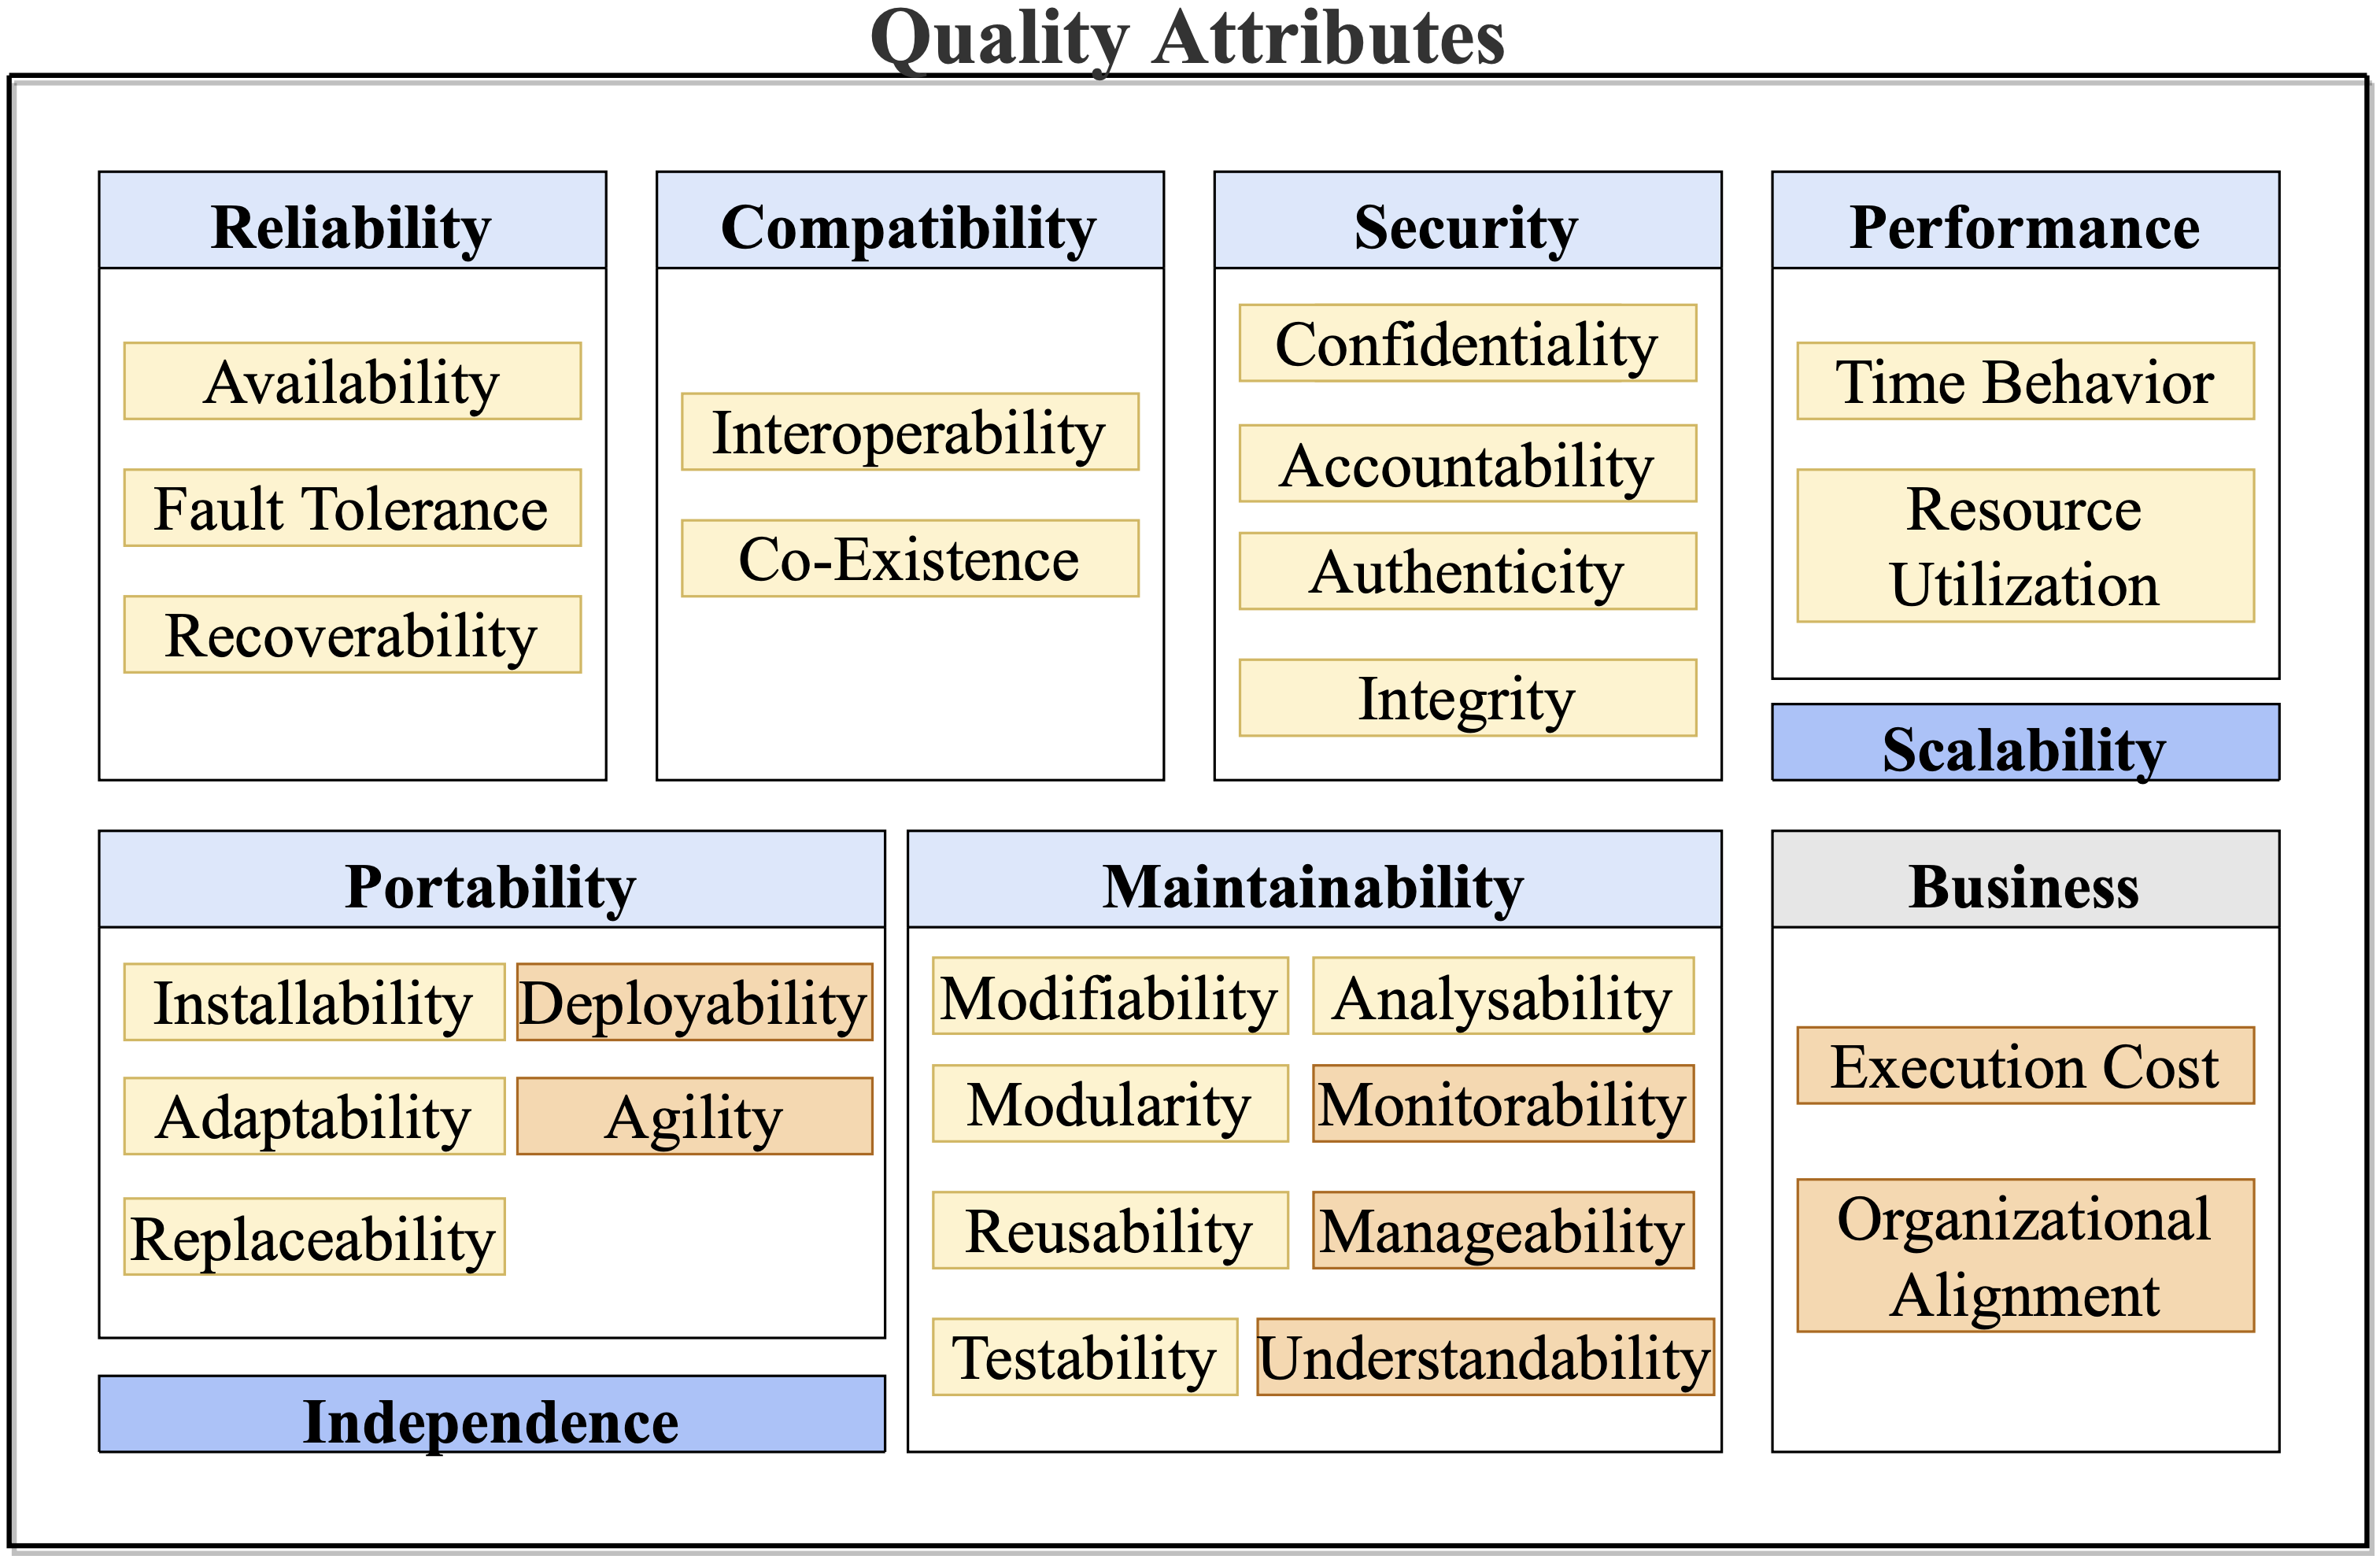
\includegraphics[width=0.8\textwidth]{qas}
	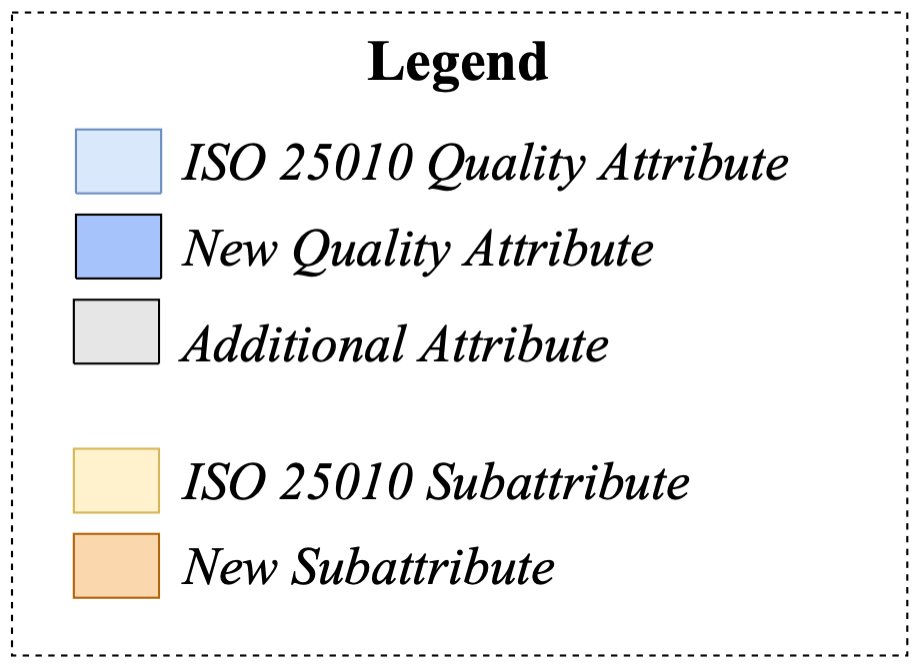
\includegraphics[width=0.3\textwidth]{qas-legend.drawio}
	\caption[Spezielle \acrlongpl{qa} für Microservices-Architekturen]{
		Spezielle \acrfullpl{qa} für Microservices-Architekturen nach \Citet{master-daniel-koch}.
	}
	\label{fig:qas}
\end{figure}
Dabei handelt es sich zu großen Teilen um die nach der Literaturrecherche wichtigsten \glspl{qa} aus der ISO 25010~\cite{ISO-25010}, die durch wenige Microservices-spezifische \glspl{qa} ergänzt wurden.
Durch die Verwendung des \gls{arh} ist die einzig sinnvolle Option, diese zu verwenden, da der \gls{arh} nur die Eingabe dieser erlaubt.

Die im zweiten Schritt erstellte Priorisierung der \glspl{qa} wird im dritten Schritt dann verwendet, um Szenarien zu erstellen.
Dieser ist in drei Sub-Schritte unterteilt:
Erst werden für die wichtigsten \glspl{qa} Szenarien erstellt.
Diese werden in Form eines Utility festgehalten (siehe \cref{fig:utility-tree}).
Dann wird jedes Szenario erneut betrachtet und eine Bewertung hinsichtlich der Wichtigkeit und technischen Schwierigkeit vorgenommen.
Diese erfolgt auf einer Skala von A bis C, wobei A für die höchste Wichtigkeit und höchste technische Schwierigkeit steht.
Abschließend wird jedes Szenario ein drittes Mal betrachtet und die Assoziation mit anderen \glspl{qa} diskutiert und festgehalten.
Bei diesem Schritt stammt nur der erste Teil aus der Methodik von \Citet{SVAHNBERG20071893} und die anderen beiden Schritte stammen aus dem \gls{arh}.
Dass bei der Vorlage von \Citet{SVAHNBERG20071893} keine vergleichbare Bewertung der Szenarien und Assoziation der Szenarien mit weiteren \glspl{qa} beschrieben ist, liegt vermutlich am Kontext des Architekturreviews.
Im Kontext der qualitativen Bewertung durch Menschen sind diese nicht explizit notwendig.
Im Vergleich dazu können bei der automatisierten Auswertung durch ein Werkzeug wie den \gls{arh} die Szenarien nicht selbstständig eingeschätzt werden.
Außerdem stammt die Visualisierung durch einen Utility Tree aus \gls{atam} \cite{kazman_2000}.
Ein solcher soll dabei helfen, Qualitätsziele zu konkretisieren und priorisieren~\cite{kazman_2000}.
Dabei werden nach einem semantisch unbedeutenden Wurzelknoten von links nach rechts die \glspl{qa} in Sub-\glspl{qa} verfeinert, worauf dann auf dritter Ebene Szenarien folgen.
Wie in \cref{fig:utility-tree} zu sehen ist, enthält die in dieser Thesis verwendete Notation des Utility Trees auch die Einschätzung der Szenarien in Wichtigkeit und technische Schwierigkeit.
\begin{figure}[!h]
	\centering
	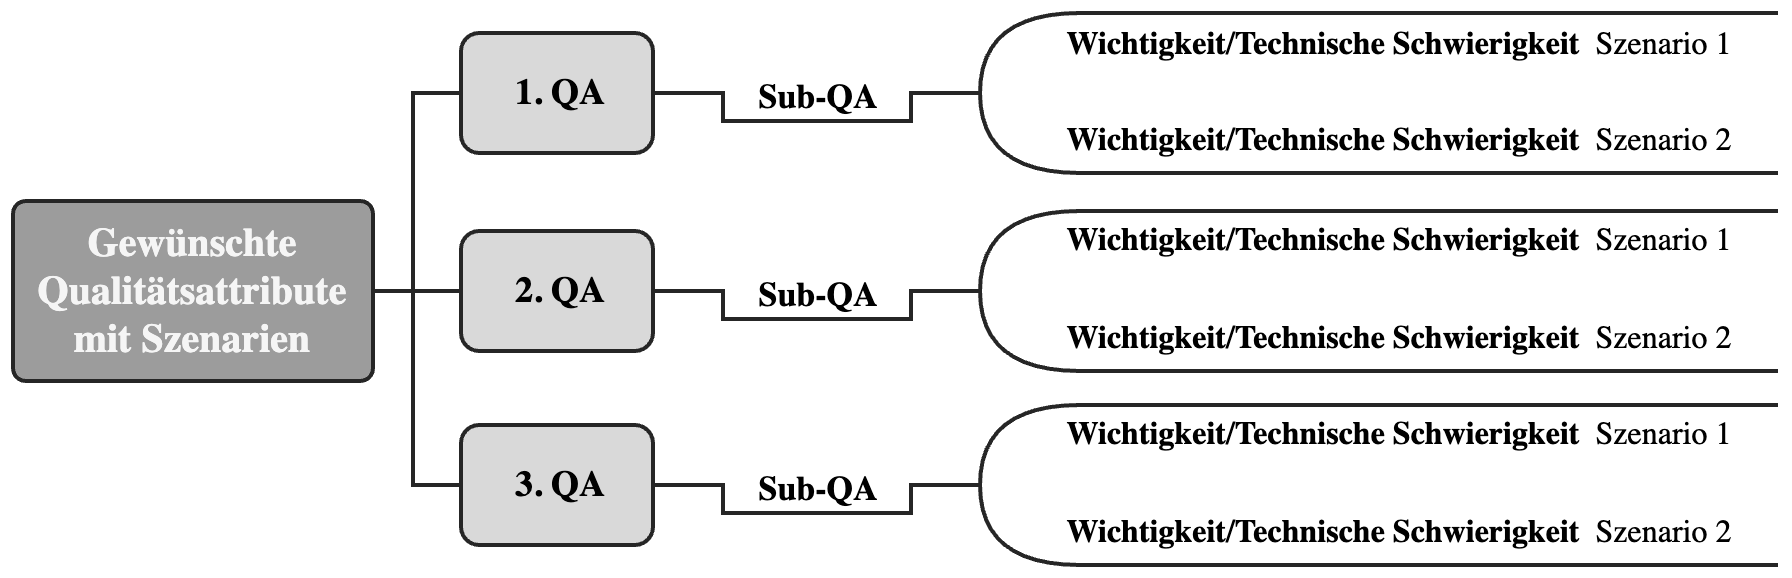
\includegraphics[width=\textwidth]{utility-tree.drawio}
	\caption[Utility Tree nach \gls{atam} \cite{kazman_2000}]{
		Utility Tree nach \gls{atam} \cite{kazman_2000} auf die Verwendung mit \gls{arh} angepasst.
	}
	\label{fig:utility-tree}
\end{figure}


Im letzten Schritt, erfolgt eine Bewertung, bei der jedem Szenario zugeordnet wird, ob eine \gls{msa} für es vorteilhaft ist.
Diese Bewertung kann als Teil des fünften Schritts nach \Citet{SVAHNBERG20071893} gesehen werden.
Abgesehen davon wird allerdings der Teil der Bewertung der Architektur unter den Szenarien im Architekturreview komplett ausgelassen und der Rest der Schritte 4, 5 und 6 nach \Citet{SVAHNBERG20071893} nicht durchgeführt.
Das liegt daran, dass während bei allen erwähnten Szenarien-basierten Verfahren die Szenarien und \glspl{qa} lediglich ein Zwischenprodukt und Mittel zu Bewertung der Architektur des Systems sind, sie im im Architekturreview, das im Rahmen dieser Thesis durchgeführt wird, das erwünschte Endprodukt darstellen.

Die vorgestellte Methodik kann als neue Methodik zur Extraktion von Szenarien und \glspl{qa} betrachtet werden und könnte in Zukunft als Vorlage für die Anwendung mit dem \gls{arh} verwendet werden.
Trotz des Mangels des Bewertungsschritts der Methodik wird sie folgend zur Vereinfachung als Architekturreview bezeichnet.

\subsection{Strukturierte Feldnotizen}
\label{sec:structured-field-notes}

Während Phase 1 also in einer Fokusgruppe durchgeführt wurde, findet die Bearbeitung in den folgenden Phasen größtenteils in Einzelarbeit statt.
Um dabei strukturiert zu protokollieren, welche Aktivitäten im Rahmen dieser Phasen durchgeführt wurden, werden systematisch durchgeführte Aktivitäten mit gemachten Erfahrungen und Herausforderungen dokumentiert und am Ende ausgewertet.
Dazu werden strukturierte Feldnotizen verwendet~\cite{seaman2008qualitative}.
Dabei können die involvierten Stakeholder zur Rate gezogen werden.


\section{Evaluation des \gls{mmf}}

Das bis inklusive Phase 3a geplante Refactoring soll dann in Phase 3b im Rahmen eines minimalen Prototyps umgesetzt und simuliert werden, da ein Refactoring des kompletten Systems im zeitlichen Rahmen dieser Arbeit nicht möglich wäre.
Dabei entstehende Prototypen könnten Vorläufer von \emph{jadice flow 2.0} werden.

Im Nachgang sollen die Ergebnisse dieses Experiments ausgewertet werden. Um quantitativ vergleichbare Ergebnisse zu erhalten, sollen im Vorlauf des Experiments Vergleichskriterien und Messmethoden definiert werden, die es möglich machen, gleichartige Anwendungsfälle von \emph{jadice flow 1.0} und neuen Prototypen zu vergleichen.
